\section{问题三：烘干时长的确定}
\label{sec:q3}

\subsection{模型的建立}
\label{sec:q3model}

问题三在方程层面与问题二完全相同：同一附录 3 物性、同一几何、同一初值与边界条件，故控制方程仍为式\eqref{eq:q2system}、物性仍为式\eqref{eq:app3}、定解条件仍为式\eqref{eq:initial}$\sim$\eqref{eq:robin}。本问新增的只有终点判据，因此建模工作的重点是把题目语言精确地翻译为一个可计算的数学问题。

题目要求``药材各处的水分浓度应低于 $0.15$~kg/kg''。定义全场最大含水率

\begin{equation}
M(\t):=\max_{0\le \rpos\le \Rzero}\C(\rpos,\t),
\label{eq:M}
\end{equation}
则``各处达标''等价于 $M(\t)<0.15$。由于水分由内向外扩散，$\C$ 沿半径单调递减（该性质在图~\ref{fig:q1C} 与交付文件中逐行可验），最慢达标的位置是轴心，故按最大值理解\textbf{既是最保守的选择，也与物理机制一致}。于是烘干时长定义为

\begin{equation}
\tend:=\min\left\{\t>0:\ M(\t)<0.15~\mathrm{kg/kg}\right\}.
\label{eq:tend}
\end{equation}

$M(\t)$ 是有限个连续函数的最大值，故本身连续，但在``最大值由哪个节点取得''切换处不可微。因此 $\tend$ 唯一且可用过零定位，但不能用 Newton 类方法，只能用依赖函数值符号的方法。

最后需要明确\textbf{判据的作用域}：判据是对物理量 $M$ 的判断，因此必须定义在求解状态（内部网格的未舍入值）上。若把判据定义在交付网格或舍入后的表格上，答案会随输出格式而变（见第~\ref{sec:q3result} 节的实测说明），这一点是本文与``直接读表格找第一个小于 $0.15$ 的行''的做法之间的本质区别。

\subsection{模型的求解}
\label{sec:q3solve}

\subsubsection{单次积分加事件检测}

把式\eqref{eq:tend} 的求根问题交给常微分方程积分器的事件机制处理：在式\eqref{eq:semi} 的半离散系统上附加事件函数

\begin{equation}
g(\t):=M(\t)-0.15,
\label{eq:event}
\end{equation}
并令积分器在 $g$ 出现\textbf{向下过零}（即 $g$ 由正变负）时记录该时刻并终止积分。这一做法的代价很低：事件检测只在每个已接受的时间步内部分辨率上做一次标量求根，不额外增加状态维数，也不需要重启积分；与二分法相比，它把``$n$ 次全程积分''降为``一次全程积分''。以本问为例，一次 $\Nr=2561$ 的全程求解约需 \QThreeWallS~s，若用二分法达到同样的时刻精度则需要十余次全程求解，代价成倍增加而精度并无提升。

由于 $M(\t)$ 在 $\arg\max$ 切换处不可微，事件定位的精度低于积分器在一阶导数连续情形下的表现。为此本文不依赖``事件时刻是精确根''这一假设，而是另外用两件事实支撑报出的 $\tend$：其一，事件时刻处的 $M$ 值恰为 $0.15$，其后立即严格小于 $0.15$；其二，收紧时间容差或更换时间积分方法后 $\tend$ 的变化量小于 $10^{-5}$~s 量级（第~\ref{sec:timecheck} 节）。二者的量级差保证了报出的时长在小数点后第三位（以小时计）是稳定的。

\subsubsection{两种口径与交付网格}

题目要求交付文件的时间列是等间隔的，而精确的 $\tend$ 一般落在 $60$~s 网格之间（本例 $205809.74$~s）。若把非整步行写进交付文件，会破坏``等间隔''的格式约定；若只写到 $\lfloor\tend/60\rfloor\cdot60$ 这一行，则该行尚未达标，与判据矛盾。因此本文采用如下口径：

\begin{itemize}
  \item \textbf{内部口径}：$\tend$ 记入摘要文件，作为``烘干所需时间''的答案；
  \item \textbf{交付口径}：交付文件写到首个严格合格的采样行 $\left(\lfloor\tend/\dt_{\mathrm{out}}\rfloor+1\right)\dt_{\mathrm{out}}$，保证文件中每一行的采样时刻都满足判据、且行间隔一律为 $60$~s。
\end{itemize}

本例两个时刻分别为 \QThreeEventS~s 与 \QThreeLastRowS~s，相差 \QThreeGap~s。二者都是事实，但含义不同：前者是数学问题的解，后者是交付文件的末行时刻。本文在摘要与结论中报出的是前者。

\subsubsection{算法流程}

问题三的完整求解流程如下（对应程序实现）：

\begin{enumerate}
  \item 按式\eqref{eq:gradedmesh} 生成 $\Nr=2561$ 的表面加密网格、控制体体积 $V_i$ 与界面位置；
  \item 按式\eqref{eq:initial} 置初值，并按式\eqref{eq:interp} 准备环境驱动（$t>14400$~s 取末值保持）；
  \item 在 $[0,14400]$~s 与 $[14400,\ \text{上界}]$ 两段上依次调用 BDF 积分器，容差 $2\times10^{-11}$/$2\times10^{-12}$，最大步长分别为 $30$~s 与 $60$~s，每段结束把末状态作为下一段初值（分段重启）；
  \item 每段都挂接式\eqref{eq:event} 的事件函数，方向为向下过零、触发即终止；
  \item 若事件触发，记录 $\tend$，再从 $\tend$ 续积到交付口径的末行时刻；若未在上界内触发，则报错退出而不静默输出一个``大概的结果''；
  \item 按第~\ref{sec:delivery} 节的规则采样、插值、按四位小数写出交付文件，并做质量收支审计。
\end{enumerate}

\subsection{结果与分析}
\label{sec:q3result}

\subsubsection{烘干时长}

\begin{equation}
\boxed{\ \tend=\QThreeEventS~\mathrm{s}=\QThreeEventH~\mathrm{h}\ }
\end{equation}

即在本模型的假设下，药材需要约 \textbf{\QThreeEventH~h}（约 $2.38$ 天）才能达到``各处水分浓度低于 $0.15$~kg/kg''的要求。交付文件 \texttt{result3.xlsx} 写到 \QThreeLastRowS~s（\QThreeLastRowH~h），文件末行的全场最大含水率为 $0.1500$~kg/kg（未舍入值 $0.14999$~kg/kg，严格合格）。事件时刻的温度场为全场 $323.315$~K，即与环境同温；事件时刻的表面含水率为 \QThreeSurfaceEnd~kg/kg，已接近环境参考值 $0.04986$~kg/kg。

按题目表 5 格式整理的结果见表~\ref{tab:q3-moisture}。

\geninput{tab/q3_moist}{表 5 由 \texttt{make tables} 从 \texttt{results/tables/q3\\_moist.csv} 生成；最后一行是烘干结束时刻。}

\subsubsection{为什么答案不是一个``凑出来''的数}

表~\ref{tab:q3-moisture} 中最后两行的中心含水率分别显示为 $0.1535$（$54$~h）与 $0.1500$（结束时刻），看上去``早一小时就该达标''；实际上这是因为干燥最后阶段的含水率变化极慢：由表~\ref{tab:scale}，当 $\C\to0.15$ 时扩散系数已降到 $8.05\times10^{-10}$~m$^2$/s，扩散特征时间达 $138$~h，远大于剩余时间。因此最后 $0.0035$~kg/kg 的下降耗时约 $3.2$~h，这是\textbf{物理规律而非数值问题}。同理，交付文件中 $t=\QThreeLastRowS$~s 与其前一行（相差 $60$~s）的中心含水率在四位小数下都显示 $0.1500$，仅凭交付文件无法判断哪一行达标——这正是第~\ref{sec:q3model} 节强调``判据必须定义在内部未舍入值上''的原因。

\subsubsection{时空分布与干燥分区}

\begin{figure}[!ht]
  \centering
  \IfFileExists{figs/fig-moist-2d.pdf}{%
    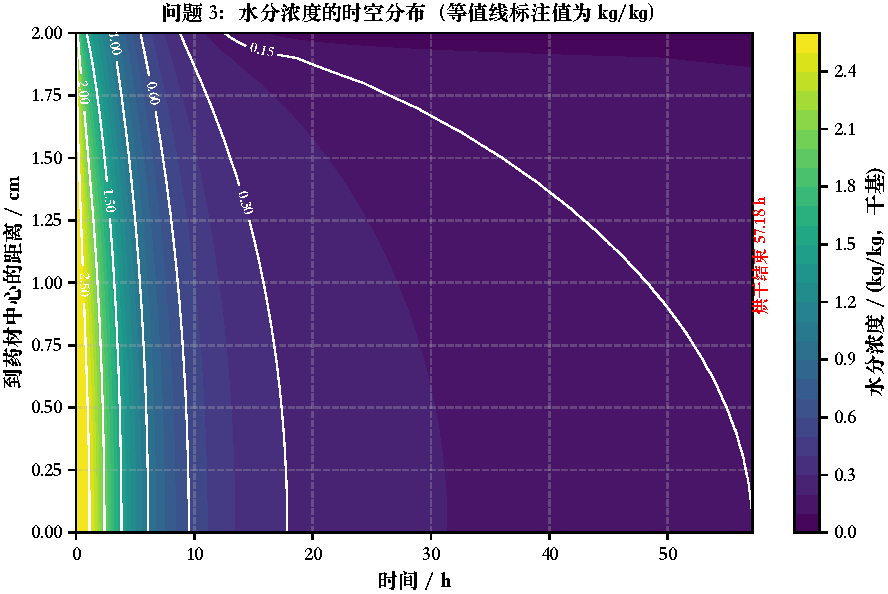
\includegraphics[width=0.49\linewidth]{figs/fig-moist-2d.pdf}%
  }{%
    \instruction{【插图缺失】未找到 \texttt{figs/fig-moist-2d.pdf}，请先运行 \texttt{make figs}。}%
  }
  \caption{问题三水分浓度的时空分布（横轴为时间、纵轴为到药材中心的距离，等值线标注值的单位为 kg/kg；红色虚线为烘干结束时刻）}
  \label{fig:q3-2d}
\end{figure}

图~\ref{fig:q3-2d} 把整个烘干过程的含水率场画在一张图上，可以清楚看到三个区域：左上方的``干燥区''（$\C<0.15$）在 $12$~h 内即从表面扩展到 $1$~cm 附近；中部的``过渡区''随着时间向内推进并逐渐变窄；右下方的``湿芯区''在 $24$~h 后才开始明显收缩，到结束时刻只剩下中心附近的窄带。整张图呈现明显的\textbf{``角点效应''}：靠近表面与长时间的组合区域含水率最低，靠近轴心与短时间的组合区域含水率最高，二者之间由一族近似平行的等值线相连。这一图形结构说明\textbf{干燥前沿是沿半径方向匀速推进的}，而不是``整体均匀失水''。

\genfig[0.60\linewidth]{figs/fig3-C-profiles.pdf}{长时间干燥下水分浓度沿半径的分布（问题三，取 $10\%$、$30\%$、$60\%$ 与 $100\%$ 干燥时长）}{fig:q3C}
\genfig[0.60\linewidth]{figs/fig3-C-history.pdf}{五个径向位置的水分浓度随时间的变化（问题三）}{fig:q3Chistory}

图~\ref{fig:q3C} 给出四个时刻的径向剖面：早期（$10\%$ 时长，约 $5.7$~h）剖面是``内部平台 $+$ 近表面陡降''；中期（$30\%$、$60\%$ 时长）剖面逐渐整体下移并趋于平直；到结束时刻剖面几乎是一条水平线（中心 $0.15$、表面 $0.0525$~kg/kg），径向差仅 $0.0975$~kg/kg。这与此前``后期由内部扩散控制''的判断一致：当内部补充速度足够慢时，断面上各点的含水率会以相同的速率缓慢下降，剖面的形状不再改变。

图~\ref{fig:q3Chistory} 从时间维度给出各位置的达标顺序：$r=2.0$~cm 的表面在 $12$~h 内就已低于 $0.15$~kg/kg，$r=1.5$~cm 在 $36$~h 附近达标，$r=1.0$~cm 在 $48$~h 后达标，而 $r=0.5$~cm 与轴心直到最后时刻才达标。因此\textbf{整个烘干时长实际上是由轴心附近最后 $0.5$~cm 的``湿芯''决定的}：从 $r=2.0$~cm 达标到轴心达标之间隔了约 $45$~h，占总时长的 $79\%$。这一观察对工艺优化有直接含义：若要缩短烘干时间，应设法提高\textbf{内部}水分的迁移能力（例如提高温度以增大扩散系数、或采用间歇式干燥让内部水分有时间重新分布），而不是单纯加大表面风速或提高表面换热强度。
